%!TEX root = ../main.tex
%%%%%%%%%%%%%%%%%%%%%%%%%%%%%%%%%%
% Links:
%
% Difficulty: Companies: 
%%%%%%%%%%%%%%%%%%%%%%%%%%%%%%%%%%

\chapter{Reverse a singly linked list}
\label{ch:list_reverse}

\section*{Introduction}
In this chapter we are going to have a look at a problem based on reversing a singly linked list. Despite the fact that this is one of the fundamental structures in computer science and is also an extremely popular interview question, it often trips up prospective candidates and is usually a cause for immediate rejection. As such, it is worth spending a bit of time on it to ensure a solid grasp of the optimal solutions. 

The problem has  a simple definition as all it asks us to do is reverse a given list.
We will discuss how we can approach this problem both a recursive and an iterative
manner. We will also examine a slightly harder variation that is
often asked as a follow-up although we leave the solution to that one for the reader. 


\section{Problem statement}
\begin{exercise}
Create a function that,  given a singly linked list $L$, reverses it and return the pointer to the new
head of $L$. $L$ is given as a pointer to the first node of the list. The definition of the node is
given in Listing \ref{list:list_reverse:node_definition}.



\begin{example}
	\hfill \\
	Given the $L = 1 \rightarrow 2 \rightarrow 3 \rightarrow 4 \rightarrow 5$, the function modifies
	it into $L = 5 \rightarrow 4 \rightarrow 3 \rightarrow 2 \rightarrow 1$ and returns a pointer to
	the node $5$, the new head of the list.
\end{example}

\end{exercise}

\lstinputlisting[language=c++, caption={Singly linked-list node definition.},label=list:list_reverse:node_definition]{sources/cycle_in_list/linked_list.h}

\section{Clarification Questions}

\begin{QandA}
	\item \begin{questionitem} \begin{question} Can the input list be empty?   \end{question} 	 
    \begin{answered}
		\textit{Yes.}
	\end{answered} \end{questionitem}

	\item \begin{questionitem} \begin{question} Can I assume $L$ is not corrupted by e.g. containing cycles?   \end{question} 	 
    \begin{answered}
		\textit{Yes, the input list is a singly linked list with no cycles.}
	\end{answered} \end{questionitem}
	
\end{QandA}

\section{Discussion}
\label{list_reverse:sec:discussion}
Solving this problem using linear additional space is trivial as we can iterate over the list
and for each push the address of each of its nodes in a stack. We can then pop them one at a time
while making sure they are connected in the same order they are popped out. Listing
\ref{list:list_reverse:stack} shows a possible implementation of this idea. The time and space
complexity of this approach is $O(n)$.

\lstinputlisting[language=c++, caption={Linear time and space complexity solution using a stack to reverse the nodes in the list.},label=list:list_reverse:stack]{sources/list_reverse/list_reverse_solution1.cpp}

We can,  however,  avoid using additional space in the form of a \inline{std::stack} and rely on the
implicit stack we get when we perform recursive calls. In order to take advantage of it, however, it is 
convenient to shift our view of the problem as follows:

Imagine we have a list such that it is already reversed after its $k^{th}$ node. How can we then reverse the rest of it?
Let's have a look at Figure \ref{fig:list_reverse:list_reverse_recursive_intermediate} depicting
this scenario where $k=4$. As we can see the list is already reversed from node $5$ onwards and all
we have to do is to have it pointing to node $4$ and make $4$ point to nothing. More generically
what we want to achieve is to make the node $k+1$ ($L_{k+1}$) point to the node $k$ ($L_{k+1}$). We
can achieve this by doing: $L_{k} \rightarrow next \rightarrow next= L_{k}(L_{k+1}$). With regard to  Figure
\ref{fig:list_reverse:list_reverse_recursive_intermediate} $L_{k} \rightarrow next$ is $5$ and
$L_{k} \rightarrow next$ is pointing to nothing. After these operations what we are left with is the
list  shown in Figure \ref{fig:list_reverse:list_reverse_recursive_intermediate1}. If we do that for
each of the nodes eventually we are left with a reversed list. 

\begin{figure}
	\vspace*{-0.5in}
	\centering
	\begin{subfigure}[t]{0.49\textwidth}
		\centering
		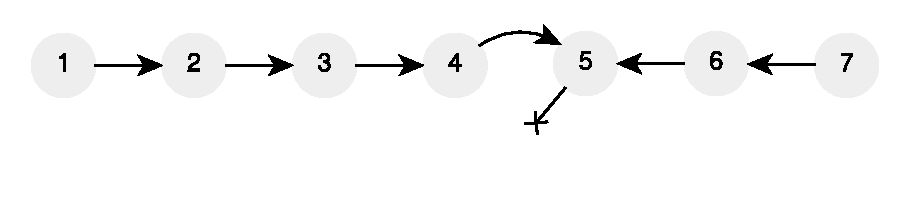
\includegraphics[width=\textwidth]{sources/list_reverse/images/list_reverse_recursive_intermediate}
		\caption[]{Nodes arrangements in the middle of the recursive process for node $5$}
		\label{fig:list_reverse:list_reverse_recursive_intermediate}
	 \end{subfigure}
	\hfill
	\begin{subfigure}[t]{0.49\textwidth}
		\centering
	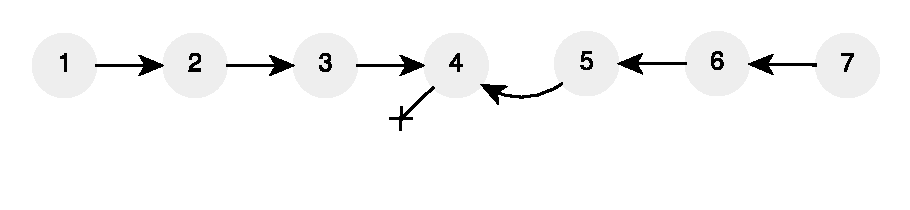
\includegraphics[width=\textwidth]{sources/list_reverse/images/list_reverse_recursive_intermediate1}
	\caption[]{Nodes arrangements after performing the recursive call for node $5$.}
	\label{fig:list_reverse:list_reverse_recursive_intermediate1}
	 \end{subfigure}
\end{figure}

But what about the new head of the list? What should each recursive call return? This is actually
fairly straightforward. Whenever we reach the end of the list\footnote{Which is when either the current node
is null or the current node does not have any node next to it.} we return the current node -  which is
effectively the new head of the reversed list -  and we keep propagating that value for all the
recursive calls. 

To summarise, for each recursive call we first reverse the rest of the list and we get back the head
of the reversed list. We can now take care of reversing the link from the current node to the next
and return the head we got back from the recursive call. Listing \ref{list:list_reverse:recursive}
shows a possible implementation of this idea. Note that despite this solution not explicitly
using any additional space, it still requires spaces for the activation frames of all the recursive
calls. As such,  its complexity remains equivalent to the one in Listing \ref{list:list_reverse:stack}.

\lstinputlisting[language=c++, caption={Recursive linear time and space complexity solution to reverse the nodes in the list.},label=list:list_reverse:recursive]{sources/list_reverse/list_reverse_solution3.cpp}

\subsection{Constant space}
It is impossible to solve this problem faster than linear time as each node must be accessed at least
once; but we can bring the space complexity down to constant. We do this by reversing the list, two nodes at a
time,  from the head to the tail. Assuming $L$ has at least two nodes (if not we are in a trivial case
in which the list is already reversed and $L$ is also the head of the reversed list) then we can
always maintain two pointers to the current element \inline{curr}and its next \inline{curr\_next}. We know that
\inline{curr}points to \inline{curr\_next} but what we really want to achieve is \inline{curr\_next} pointing to $curr$.
We can take care of that and proceed with moving curr and \inline{curr\_next} forward and repeat the process.
Eventually we will have reversed all nodes in the list. This process ends whenever we reach the last node
of the list; which also happen to be the new head of the list.

An implementation of such idea is shown in Listing \ref{list:list_reverse:constant_space}. Note
that while making \inline{curr\_next} point to \inline{curr}we must also remember the element
\inline{curr\_next} points to, otherwise it would be impossible to move \inline{curr} and
\inline{curr\_next} forward.
Figure \ref{fig:list_reverse:list_reverse_iterative_execution} shows the execution of the algorithm in Listing \ref{list:list_reverse:constant_space} on a list of $7$ elements.


\lstinputlisting[language=c++, caption={Iterative constant space solution to the problem of reversing a list. },label=list:list_reverse:constant_space]{sources/list_reverse/list_reverse_solution2.cpp}

\begin{figure}
	\vspace*{-0.5in}
	\centering
	\begin{subfigure}[t]{0.49\textwidth}
		\centering
		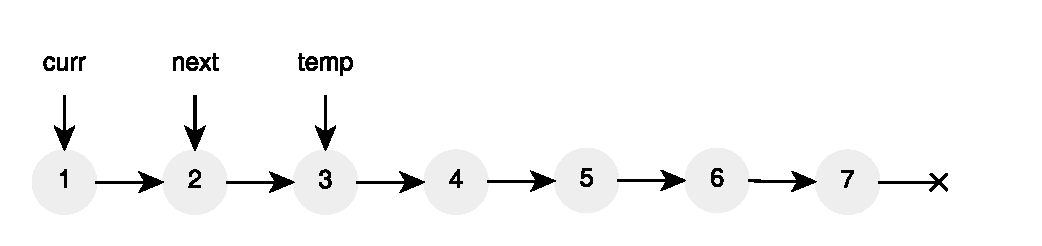
\includegraphics[width=\textwidth]{sources/list_reverse/images/list_reverse_iterative1}
		\caption[]{Step $1$}
		\label{fig:list_reverse:list_reverse_iterative1}
	 \end{subfigure}
	\hfill
	\begin{subfigure}[t]{0.49\textwidth}
		\centering
		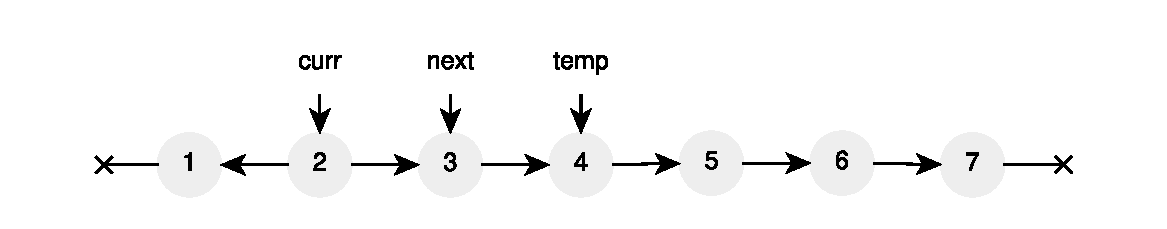
\includegraphics[width=\textwidth]{sources/list_reverse/images/list_reverse_iterative2}
		\caption[]{Step $2$}
		\label{fig:list_reverse:list_reverse_iterative2}
	 \end{subfigure}
	 \hfill
	 \begin{subfigure}[t]{0.49\textwidth}
		\centering
		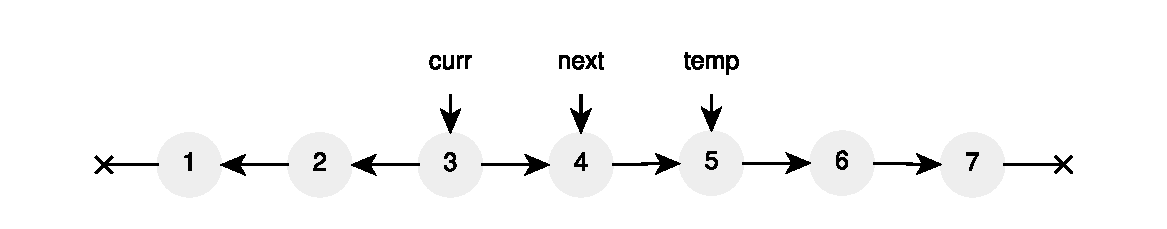
\includegraphics[width=\textwidth]{sources/list_reverse/images/list_reverse_iterative3}
		\caption[]{Step $3$}
		\label{fig:list_reverse:list_reverse_iterative3}
	 \end{subfigure}
	 \hfill
	 \begin{subfigure}[t]{0.49\textwidth}
		\centering
		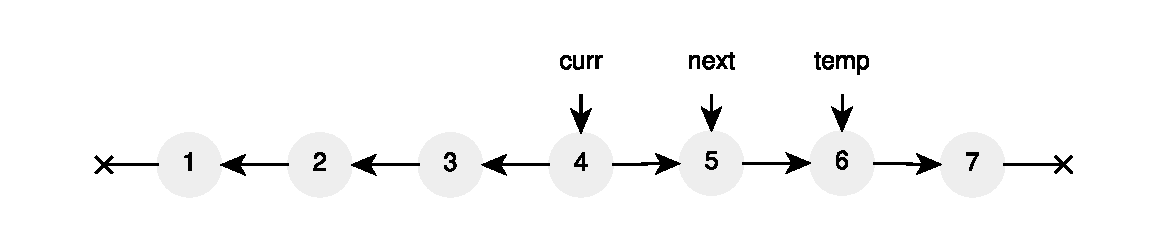
\includegraphics[width=\textwidth]{sources/list_reverse/images/list_reverse_iterative4}
		\caption[]{Step $4$}
		\label{fig:list_reverse:list_reverse_iterative4}
	 \end{subfigure}
	 \hfill
	 \begin{subfigure}[t]{0.49\textwidth}
		\centering
		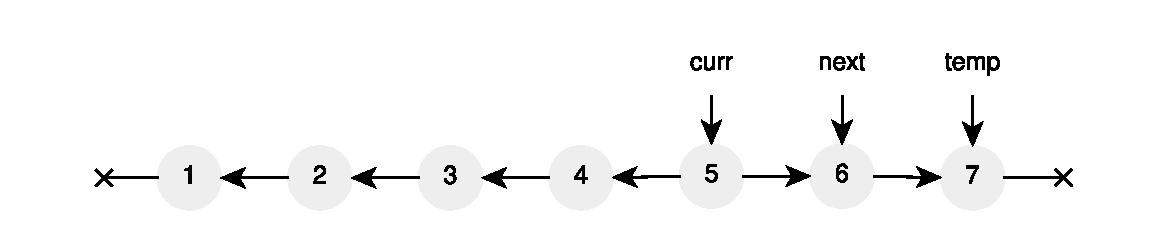
\includegraphics[width=\textwidth]{sources/list_reverse/images/list_reverse_iterative5}
		\caption[]{Step $5$}
		\label{fig:list_reverse:list_reverse_iterative5}
	 \end{subfigure}
	 \hfill
	 \begin{subfigure}[t]{0.49\textwidth}
		\centering
		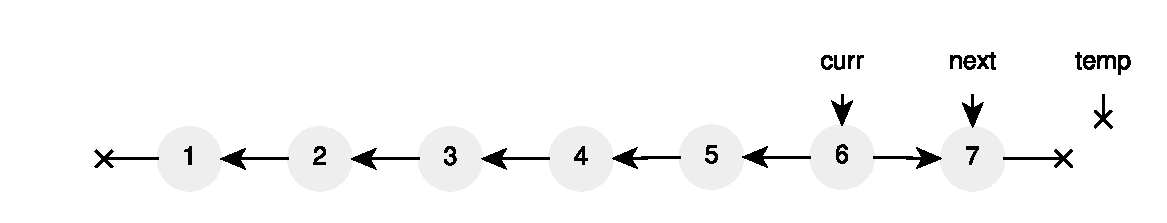
\includegraphics[width=\textwidth]{sources/list_reverse/images/list_reverse_iterative6}
		\caption[]{Step $6$}
		\label{fig:list_reverse:list_reverse_iterative6}
	 \end{subfigure}
	 \hfill
	 \begin{subfigure}[t]{0.49\textwidth}
		\centering
		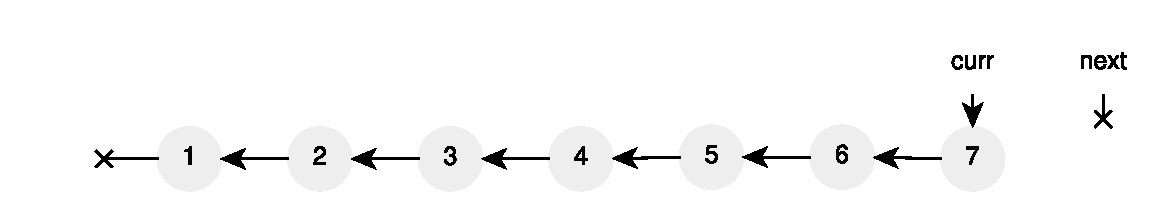
\includegraphics[width=\textwidth]{sources/list_reverse/images/list_reverse_iterative7}
		\caption[]{Step $7$. \inline{curr} is the new head of the reversed list.}
		\label{fig:list_reverse:list_reverse_iterative7}
	 \end{subfigure}
\caption{Execution of the algorithm implemented in Listing \ref{list:list_reverse:constant_space} on the list $L = 1 \rightarrow 2 \rightarrow 3 \rightarrow 4 \rightarrow 5 \rightarrow 6 \rightarrow 7$}
\label{fig:list_reverse:list_reverse_iterative_execution}
\end{figure}

\section{Conclusion}
We have discussed three possible approaches to the problem of reversing a singly-linked list.
We saw that it is almost trivial when using an iterative approach together with a stack to store the addressed of the list's nodes. 
This approach is based on the fact that the ordering of $n$  elements popped from a stack is the reverse of the ordering the elements have been pushed on to.

We then examined an alternative solution that, whilst based based on the same stack idea, does not use an explicit stack to store the nodes but rather stores the same information in the 
call stack of the recursive function. 

Finally,  we discussed a solution where only a constant space is required. This approach works iteratively from the head to the tail of the list by reversing two nodes at a time.

\section{Common variation - Reverse a sublist}
\subsection{Problem statement}
\begin{exercise}
Create a function that,  given a singly linked list $L$ and two integers $n \geq  m \geq 0$,
reverses only its nodes from the $m^{th}$ to the $n^{th}$ and return the pointer to the new
head of $L$. As in the other version of this problem discussed above the definition of a node is the same and the list 
$L$ is given as a pointer to the first node of the list itself.

\begin{example}
	\hfill \\
	Given the $L = 1 \rightarrow 2 \rightarrow 3 \rightarrow 4 \rightarrow 5$, $m = 3$, $n = 5$ the function modifies
	it into $L = 1 \rightarrow 2 \rightarrow 5 \rightarrow 4 \rightarrow 3$ and returns a pointer to
	the node $1$.
\end{example}

\begin{example}
	\hfill \\
	Given the $L = 1 \rightarrow 2 \rightarrow 3 \rightarrow 4 \rightarrow 5$, $m = 1$, $n = 2$ the function modifies
	it into $L = 1 \rightarrow 2 \rightarrow 5 \rightarrow 4 \rightarrow 3$ and returns a pointer to
	the node $1$.
\end{example}

\end{exercise}
